\documentclass{standalone}
\usepackage{tikz}
\usetikzlibrary{patterns}
\usetikzlibrary{positioning}
\usetikzlibrary{patterns, positioning}
\usetikzlibrary{shapes.misc}
\usepackage[outline]{contour}
\contourlength{1.5pt} 
\usepackage[sfdefault]{ClearSans}

\begin{document}
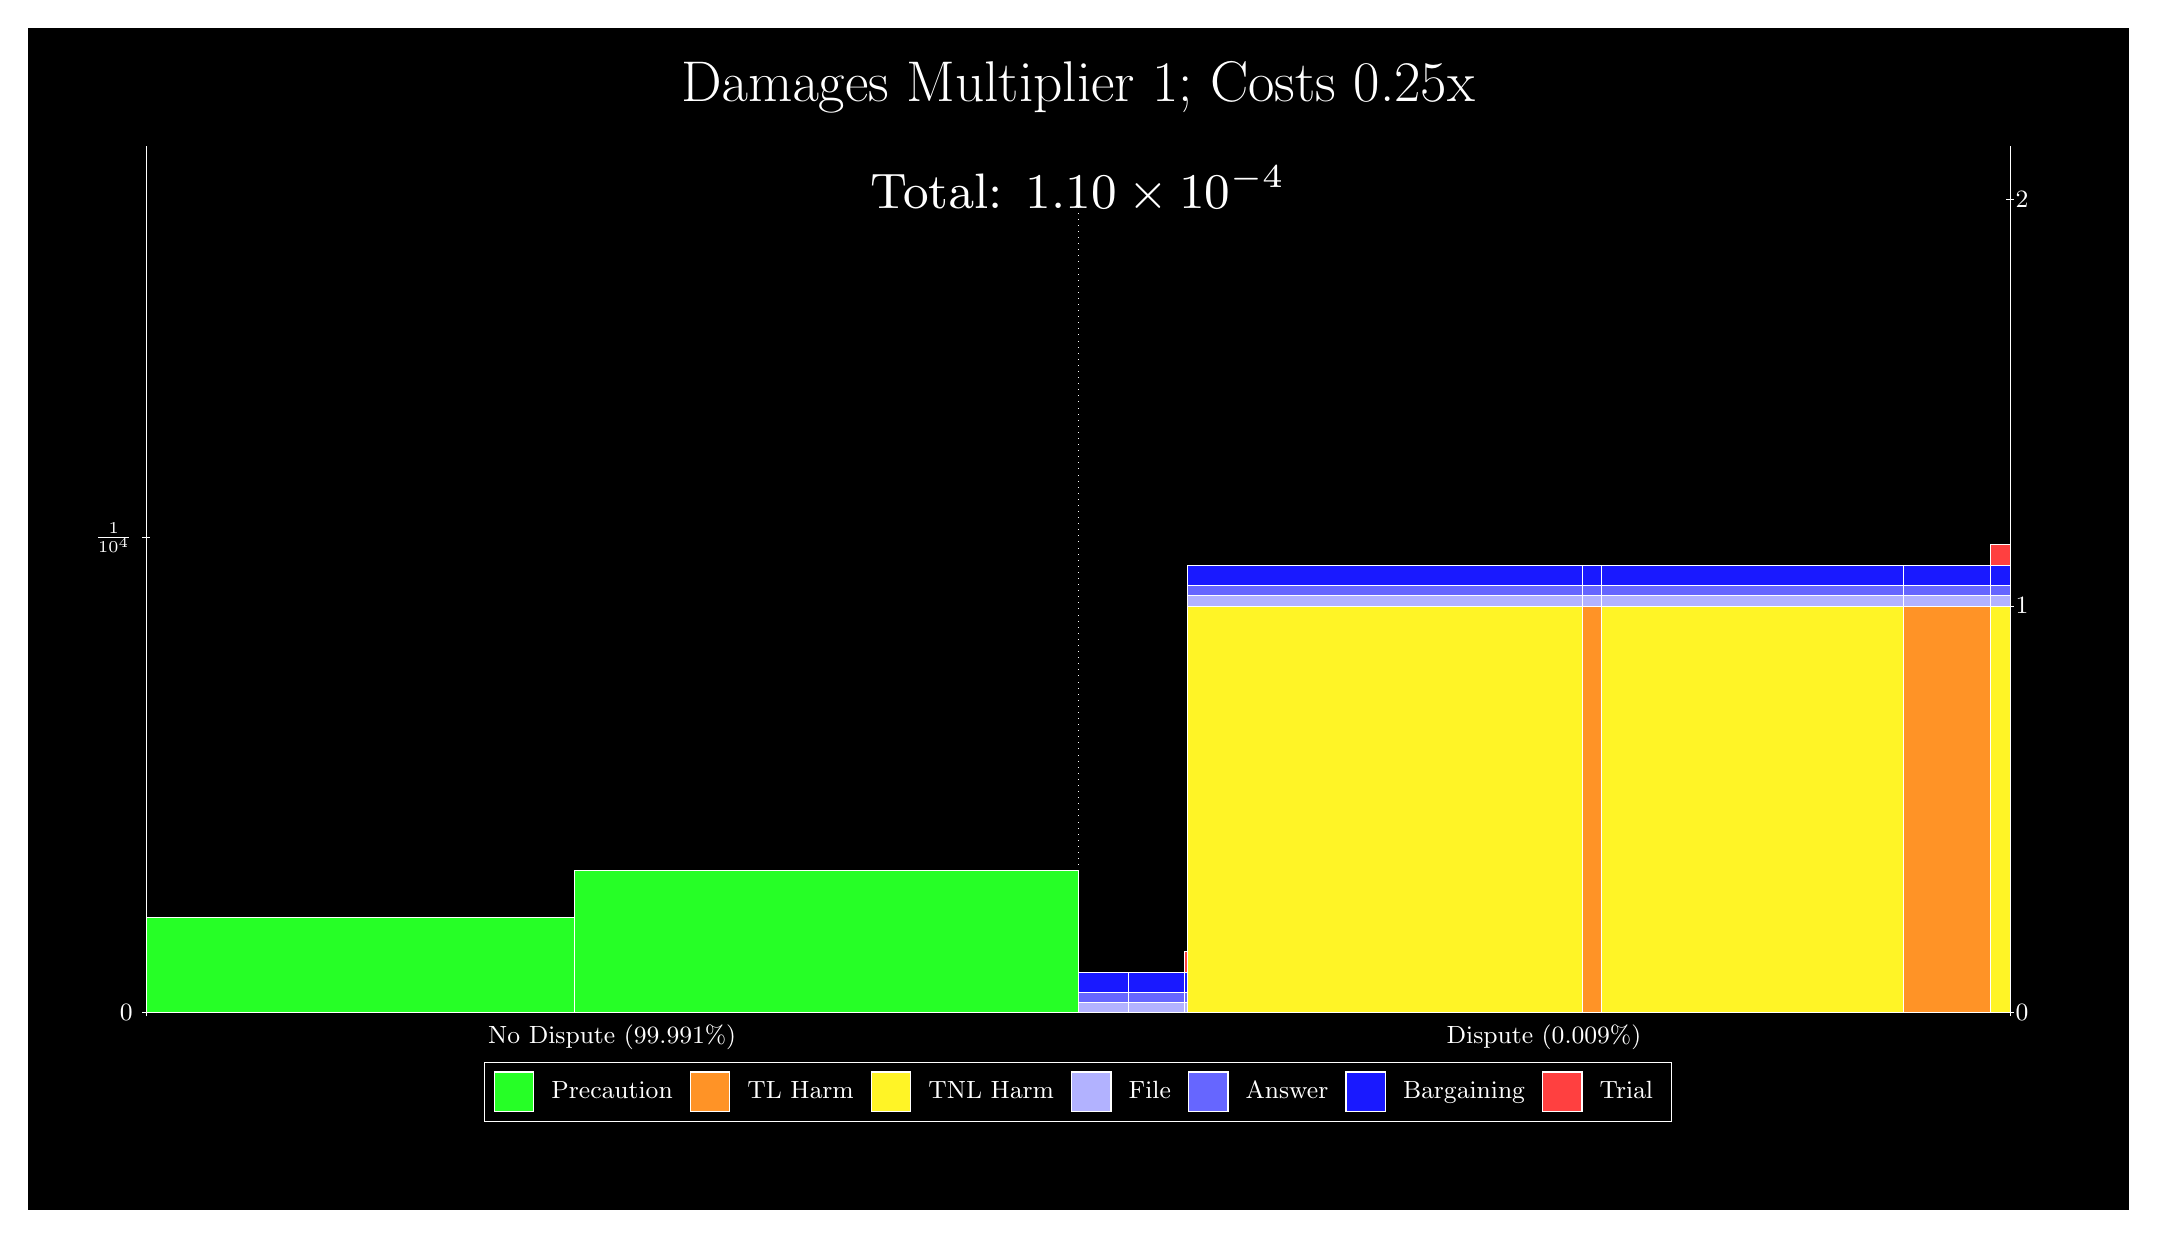
\begin{tikzpicture}
\draw[fill=black] (0,0) rectangle (26.667,15);
\draw[draw=none,text=white] (0,13.5) rectangle (26.667,15) node[midway] {\huge Damages Multiplier 1; Costs 0.25x};
\draw[fill=green!85,draw=white,very thin] (1.5,2.5) rectangle (6.9352,3.7059);
\draw[fill=green!85,draw=white,very thin] (6.9352,2.5) rectangle (13.333,4.3088);
\draw[fill=green!85,draw=white,very thin] (13.333,2.5) rectangle (13.967,2.5001);
\draw[fill=blue!30,draw=white,very thin] (13.333,2.5001) rectangle (13.967,2.6292);
\draw[fill=blue!60,draw=white,very thin] (13.333,2.6292) rectangle (13.967,2.7583);
\draw[fill=blue!90,draw=white,very thin] (13.333,2.7583) rectangle (13.967,3.0166);
\draw[fill=green!85,draw=white,very thin] (13.967,2.5) rectangle (14.685,2.5002);
\draw[fill=blue!30,draw=white,very thin] (13.967,2.5002) rectangle (14.685,2.6293);
\draw[fill=blue!60,draw=white,very thin] (13.967,2.6293) rectangle (14.685,2.7584);
\draw[fill=blue!90,draw=white,very thin] (13.967,2.7584) rectangle (14.685,3.0166);
\draw[fill=green!85,draw=white,very thin] (14.685,2.5) rectangle (14.716,2.5002);
\draw[fill=blue!30,draw=white,very thin] (14.685,2.5002) rectangle (14.716,2.6293);
\draw[fill=blue!60,draw=white,very thin] (14.685,2.6293) rectangle (14.716,2.7584);
\draw[fill=blue!90,draw=white,very thin] (14.685,2.7584) rectangle (14.716,3.0166);
\draw[fill=red!75,draw=white,very thin] (14.685,3.0166) rectangle (14.716,3.2749);
\draw[fill=green!85,draw=white,very thin] (14.716,2.5) rectangle (19.732,2.5001);
\draw[fill=yellow!85,draw=white,very thin] (14.716,2.5001) rectangle (19.732,7.665);
\draw[fill=blue!30,draw=white,very thin] (14.716,7.665) rectangle (19.732,7.7941);
\draw[fill=blue!60,draw=white,very thin] (14.716,7.7941) rectangle (19.732,7.9232);
\draw[fill=blue!90,draw=white,very thin] (14.716,7.9232) rectangle (19.732,8.1815);
\draw[fill=green!85,draw=white,very thin] (19.732,2.5) rectangle (19.978,2.5001);
\draw[fill=orange!85,draw=white,very thin] (19.732,2.5001) rectangle (19.978,7.665);
\draw[fill=blue!30,draw=white,very thin] (19.732,7.665) rectangle (19.978,7.7941);
\draw[fill=blue!60,draw=white,very thin] (19.732,7.7941) rectangle (19.978,7.9232);
\draw[fill=blue!90,draw=white,very thin] (19.732,7.9232) rectangle (19.978,8.1815);
\draw[fill=green!85,draw=white,very thin] (19.978,2.5) rectangle (23.814,2.5002);
\draw[fill=yellow!85,draw=white,very thin] (19.978,2.5002) rectangle (23.814,7.665);
\draw[fill=blue!30,draw=white,very thin] (19.978,7.665) rectangle (23.814,7.7942);
\draw[fill=blue!60,draw=white,very thin] (19.978,7.7942) rectangle (23.814,7.9233);
\draw[fill=blue!90,draw=white,very thin] (19.978,7.9233) rectangle (23.814,8.1815);
\draw[fill=green!85,draw=white,very thin] (23.814,2.5) rectangle (24.923,2.5002);
\draw[fill=orange!85,draw=white,very thin] (23.814,2.5002) rectangle (24.923,7.665);
\draw[fill=blue!30,draw=white,very thin] (23.814,7.665) rectangle (24.923,7.7942);
\draw[fill=blue!60,draw=white,very thin] (23.814,7.7942) rectangle (24.923,7.9233);
\draw[fill=blue!90,draw=white,very thin] (23.814,7.9233) rectangle (24.923,8.1815);
\draw[fill=green!85,draw=white,very thin] (24.923,2.5) rectangle (25.167,2.5002);
\draw[fill=yellow!85,draw=white,very thin] (24.923,2.5002) rectangle (25.167,7.665);
\draw[fill=blue!30,draw=white,very thin] (24.923,7.665) rectangle (25.167,7.7942);
\draw[fill=blue!60,draw=white,very thin] (24.923,7.7942) rectangle (25.167,7.9233);
\draw[fill=blue!90,draw=white,very thin] (24.923,7.9233) rectangle (25.167,8.1815);
\draw[fill=red!75,draw=white,very thin] (24.923,8.1815) rectangle (25.167,8.4398);
\node[font=\small,text=white,anchor=north,scale=2] at (13.333, 13.5) {Total: $1.10\times 10^{-4}$};
\draw[white,very thin] (1.5,2.5) -- (1.5,13.5);
\draw[white,very thin] (1.45,2.5) -- (1.55,2.5);
\node[font=\small,text=white, anchor=east] at (1.45, 2.5) {0};
\draw[white,very thin] (1.45,8.5295) -- (1.55,8.5295);
\node[font=\small,text=white, anchor=east] at (1.45, 8.5295) {$\frac{1}{10^{4}}$};

\draw[white,dotted,very thin] (13.333,2.83) -- (13.333,13.17);
\draw[white,very thin] (25.167,2.5) -- (25.167,13.5);
\draw[white,very thin] (25.117,2.5) -- (25.217,2.5);
\node[font=\small,text=white, anchor=west] at (25.117, 2.5) {0};
\draw[white,very thin] (25.117,7.6649) -- (25.217,7.6649);
\node[font=\small,text=white, anchor=west] at (25.117, 7.6649) {1};
\draw[white,very thin] (25.117,12.83) -- (25.217,12.83);
\node[font=\small,text=white, anchor=west] at (25.117, 12.83) {2};

\draw[white,very thin] (1.5,2.5) -- (25.167,2.5);
\draw[white,very thin] (1.5,2.45) -- (1.5,2.55);
\node[font=\small,text=white, anchor=north] at (1.5, 2.45) {};
\draw[white,very thin] (25.167,2.45) -- (25.167,2.55);
\node[font=\small,text=white, anchor=north] at (25.167, 2.45) {};

\node[font=\small,text=white,anchor=south] at (7.4167, 1.9) {No\ Dispute\ (99.991\%)};
\node[font=\small,text=white,anchor=south] at (19.25, 1.9) {Dispute\ (0.009\%)};
\draw (13.3333,2.5) node (B) {};
\begin{scope}[align=center]
\matrix[scale=0.5,draw=white,below=0.5cm of B,nodes={draw},column sep=0.1cm]{
\node[rectangle,draw,minimum width=0.5cm,minimum height=0.5cm,fill=green!85]{}; & \node[draw=none,font=\small,text=white]{Precaution}; &
\node[rectangle,draw,minimum width=0.5cm,minimum height=0.5cm,fill=orange!85]{}; & \node[draw=none,font=\small,text=white]{TL Harm}; &
\node[rectangle,draw,minimum width=0.5cm,minimum height=0.5cm,fill=yellow!85]{}; & \node[draw=none,font=\small,text=white]{TNL Harm}; &
\node[rectangle,draw,minimum width=0.5cm,minimum height=0.5cm,fill=blue!30]{}; & \node[draw=none,font=\small,text=white]{File}; &
\node[rectangle,draw,minimum width=0.5cm,minimum height=0.5cm,fill=blue!60]{}; & \node[draw=none,font=\small,text=white]{Answer}; &
\node[rectangle,draw,minimum width=0.5cm,minimum height=0.5cm,fill=blue!90]{}; & \node[draw=none,font=\small,text=white]{Bargaining}; &
\node[rectangle,draw,minimum width=0.5cm,minimum height=0.5cm,fill=red!75]{}; & \node[draw=none,font=\small,text=white]{Trial}; \\\\
};\end{scope}

\end{tikzpicture}
\end{document}